\documentclass[journal,12pt,twocolumn]{IEEEtran}
\usepackage{setspace}
\usepackage{gensymb}
\singlespacing
\usepackage[cmex10]{amsmath}
\usepackage{amsthm}
\usepackage{mathrsfs}
\usepackage{txfonts}
\usepackage{stfloats}
\usepackage{bm}
\usepackage{cite}
\usepackage{cases}
\usepackage{subfig}
\usepackage{longtable}
\usepackage{multirow}
\usepackage{enumitem}
\usepackage{mathtools}
\usepackage{steinmetz}
\usepackage{tikz}
\usepackage{circuitikz}
\usepackage{verbatim}
\usepackage{tfrupee}
\usepackage[breaklinks=true]{hyperref}
\usepackage{tkz-euclide}

\usetikzlibrary{calc,math}
\usepackage{listings}
    \usepackage{color}                                            %%
    \usepackage{array}                                            %%
    \usepackage{longtable}                                        %%
    \usepackage{calc}                                             %%
    \usepackage{multirow}                                         %%
    \usepackage{hhline}                                           %%
    \usepackage{ifthen}                                           %%

    \usepackage{lscape}     
\usepackage{multicol}
\usepackage{chngcntr}

\DeclareMathOperator*{\Res}{Res}
\renewcommand\thesection{\arabic{section}}
\renewcommand\thesubsection{\thesection.\arabic{subsection}}
\renewcommand\thesubsubsection{\thesubsection.\arabic{subsubsection}}

\renewcommand\thesectiondis{\arabic{section}}
\renewcommand\thesubsectiondis{\thesectiondis.\arabic{subsection}}
\renewcommand\thesubsubsectiondis{\thesubsectiondis.\arabic{subsubsection}}

\hyphenation{op-tical net-works semi-conduc-tor}
\def\inputGnumericTable{}                                 %%

\lstset{
frame=single, 
breaklines=true,
columns=fullflexible
}

\begin{document}

\newtheorem{theorem}{Theorem}[section]
\newtheorem{problem}{Problem}
\newtheorem{proposition}{Proposition}[section]
\newtheorem{lemma}{Lemma}[section]
\newtheorem{corollary}[theorem]{Corollary}
\newtheorem{example}{Example}[section]
\newtheorem{definition}[problem]{Definition}
\newcommand{\BEQA}{\begin{eqnarray}}
\newcommand{\EEQA}{\end{eqnarray}}
\newcommand{\define}{\stackrel{\triangle}{=}}
\bibliographystyle{IEEEtran}

\providecommand{\mbf}{\mathbf}
\providecommand{\pr}[1]{\ensuremath{\Pr\left(#1\right)}}
\providecommand{\qfunc}[1]{\ensuremath{Q\left(#1\right)}}
\providecommand{\sbrak}[1]{\ensuremath{{}\left[#1\right]}}
\providecommand{\lsbrak}[1]{\ensuremath{{}\left[#1\right.}}
\providecommand{\rsbrak}[1]{\ensuremath{{}\left.#1\right]}}
\providecommand{\brak}[1]{\ensuremath{\left(#1\right)}}
\providecommand{\lbrak}[1]{\ensuremath{\left(#1\right.}}
\providecommand{\rbrak}[1]{\ensuremath{\left.#1\right)}}
\providecommand{\cbrak}[1]{\ensuremath{\left\{#1\right\}}}
\providecommand{\lcbrak}[1]{\ensuremath{\left\{#1\right.}}
\providecommand{\rcbrak}[1]{\ensuremath{\left.#1\right\}}}
\theoremstyle{remark}
\newtheorem{rem}{Remark}
\newcommand{\sgn}{\mathop{\mathrm{sgn}}}
\providecommand{\abs}[1]{\left\vert#1\right\vert}
\providecommand{\res}[1]{\Res\displaylimits_{#1}} 
\providecommand{\norm}[1]{\left\lVert#1\right\rVert}

\providecommand{\mtx}[1]{\mathbf{#1}}
\providecommand{\mean}[1]{E\left[ #1 \right]}
\providecommand{\fourier}{\overset{\mathcal{F}}{ \rightleftharpoons}}

\providecommand{\system}{\overset{\mathcal{H}}{ \longleftrightarrow}}
\newcommand{\solution}{\noindent \textbf{Solution: }}
\newcommand{\cosec}{\,\text{cosec}\,}
\providecommand{\dec}[2]{\ensuremath{\overset{#1}{\underset{#2}{\gtrless}}}}
\newcommand{\myvec}[1]{\ensuremath{\begin{pmatrix}#1\end{pmatrix}}}
\newcommand{\mydet}[1]{\ensuremath{\begin{vmatrix}#1\end{vmatrix}}}
\numberwithin{equation}{subsection}

\makeatletter
\@addtoreset{figure}{problem}
\makeatother
\let\StandardTheFigure\thefigure
\let\vec\mathbf

\renewcommand{\thefigure}{\theproblem}

\def\putbox#1#2#3{\makebox[0in][l]{\makebox[#1][l]{}\raisebox{\baselineskip}[0in][0in]{\raisebox{#2}[0in][0in]{#3}}}}
     \def\rightbox#1{\makebox[0in][r]{#1}}
     \def\centbox#1{\makebox[0in]{#1}}
     \def\topbox#1{\raisebox{-\baselineskip}[0in][0in]{#1}}
     \def\midbox#1{\raisebox{-0.5\baselineskip}[0in][0in]{#1}}
\vspace{3cm}
\title{Assignment-4}
\author{Vipul Kumar Malik \\ AI20MTECH14006}

\date{\today}

\maketitle
\newpage
\bigskip
\renewcommand{\thefigure}{\theenumi}
\renewcommand{\thetable}{\theenumi}

\begin{abstract}
This document explains the concept of congruence of triangles in a quadrilateral.
\end{abstract}
Download all python codes from 
\begin{lstlisting}
https://github.com/vipulmalik8569/MT-EE5609
\end{lstlisting}
and latex-tikz codes from 
\begin{lstlisting}
https://github.com/vipulmalik8569/MT-EE5609
\end{lstlisting}
\section{\textbf{Problem}}
In quadrilateral $ACBD$, $AC = AD$ and $AB$ bisects $\angle{A}$. Show that $BC = BD$. 

\section{Figure}
\begin{figure}[!htb]
	\centering
    \centering
    \resizebox{\columnwidth}{!}{\documentclass{article}
\usepackage[utf8]{inputenc}
\usepackage{tikz}
\usetikzlibrary{positioning}
\begin{document}
	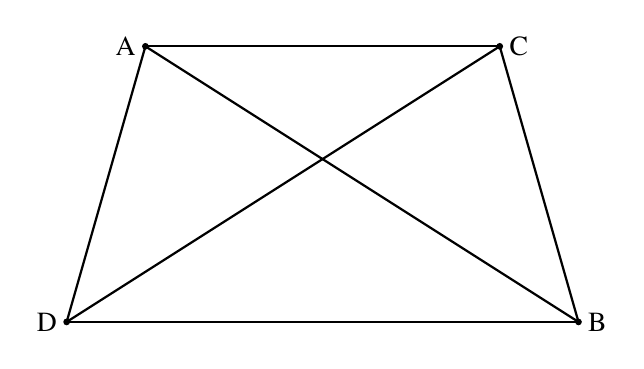
\begin{tikzpicture}
    	\draw[black, thick] (0,0) --(1,3.5); 
	\draw[black, thick] (1,3.5)--(5.5,3.5);
	\draw[black, thick] (5.5,3.5)--(6.5,0);
	\draw[black, thick] (6.5,0)--(0,0);

	\draw[black, thick] (0,0)--(5.5,3.5);
	\draw[black, thick] (1,3.5)--(6.5,0);
	
	\filldraw[black] (0,0) circle (1pt) node[anchor=east] {D};
	\filldraw[black] (6.5,0) circle (1pt) node[anchor=west] {B};
    	\filldraw[black] (5.5,3.5) circle (1pt) node[anchor=west] {C};
    	\filldraw[black] (1,3.5) circle (1pt) node[anchor=east] {A};
	\end{tikzpicture}
\end{document}
}
	\caption{Quadrilateral ACBD}
\end{figure}

\section{\textbf{Solution}}

In Quadrilateral ACBD it is given that :
\begin{align}
    AC&=AD \label{eq:1}\\ 
\angle{CAB}&=\angle{DAB} \label{eq:2}
\end{align}
By taking cosine on both sides of \eqref{eq:1} we get
\begin{align}
    \cos{\angle{CAB}}&=\cos{\angle{DAB}}\\
    \frac{(\Vec{A}-\Vec{D})^T(\Vec{A}-\Vec{B})}{\norm{\Vec{A}-\Vec{D}}\norm{\Vec{A}-\Vec{B}}} &= \frac{(\Vec{A}-\Vec{C})^T(\Vec{A}-\Vec{B})}{\norm{\Vec{A}-\Vec{C}}\norm{\Vec{A}-\Vec{B}}} \label{eq:4}
\end{align}
From \eqref{eq:1}
\begin{align}
    \norm{\Vec{A}-\Vec{D}}&=\norm{\Vec{A}-\Vec{C}}\label{eq:5}
\end{align}
Therefore \eqref{eq:4} will become 
\begin{align}
(\Vec{A}-\Vec{D})^T(\Vec{A}-\Vec{B})&=(\Vec{A}-\Vec{C})^T(\Vec{A}-\Vec{B})\label{eq:6}\\
\norm{\Vec{A}-\Vec{D}}^2-(\Vec{A}-\Vec{D})^T(\Vec{B}-\Vec{D})&=\norm{\Vec{A}-\Vec{C}}^2-(\Vec{A}-\Vec{C})^T(\Vec{B}-\Vec{C})
\end{align}
Using \eqref{eq:5} we get
\begin{align}
(\Vec{B}-\Vec{D})^T(\Vec{A}-\Vec{D})&=(\Vec{B}-\Vec{C})^T(\Vec{A}-\Vec{C})\\
\norm{\Vec{B}-\Vec{D}}^2+(\Vec{A}-\Vec{B})^T(\Vec{B}-\Vec{D})&=\norm{\Vec{B}-\Vec{C}}^2+(\Vec{A}-\Vec{B})^T(\Vec{B}-\Vec{C})\\
\norm{\Vec{B}-\Vec{D}}^2+(\Vec{A}-\Vec{D})^T(\Vec{A}-\Vec{B})&=\norm{\Vec{B}-\Vec{C}}^2+(\Vec{A}-\Vec{C})^T(\Vec{A}-\Vec{B})\label{eq:10}
\end{align}
Using \eqref{eq:6}  we get : 
\begin{align}
 \norm{\Vec{B}-\Vec{D}}^2 &= \norm{\Vec{B}-\Vec{C}}^2\\
 \norm{\Vec{B}-\Vec{D}} &= \norm{\Vec{B}-\Vec{C}}\\
 BD&=BC
\end{align}
\end{document}
